\section{Implementation Environment}

The complete experimental testbed was deployed and validated on an Apple Silicon Darwin platform (macOS 15.x, 8-core CPU, 16~GB unified RAM) using Docker-based service orchestration alongside native C++20 and Python execution runtimes. Table~\ref{tab:tech_stack} details the software stack and infrastructure components utilized across both phases.

\begin{table}[htbp]
\centering
\begin{tabular}{l l l}
\toprule
\textbf{Subsystem} & \textbf{Component / Framework} & \textbf{Version / Specification} \\
\midrule
Stream Broker        & Apache Kafka                  & 7.5 (Confluent Platform, Docker) \\
Coordination Service & Apache ZooKeeper              & 3.8 (Docker Orchestration) \\
Telemetry Blackboard & Redis In-Memory Store         & 7.2 (Alpine Linux container) \\
Query Serving API    & FastAPI + Uvicorn             & 0.110.0 (Asynchronous ASGI) \\
Python Worker        & CPython 3.11+, kafka-python-ng & mmh3 4.1.0, psutil 5.9.8 \\
C++ Worker           & Native C++20, CMake 3.28      & librdkafka 2.3.0, xxHash (XXH64) \\
Real-Time Dashboard  & HTML5, CSS3, Vanilla JS       & Chart.js 4.4.1 (WebSockets / Polling) \\
Testing Framework    & pytest 8.0, Catch2 v3         & 49 automated offline unit tests \\
\bottomrule
\end{tabular}
\caption{Software stack and experimental testbed specifications.}
\label{tab:tech_stack}
\end{table}

Underlying data services (Kafka brokers, ZooKeeper quorum, Redis instance) are containerized and orchestrated via \texttt{docker-compose.yml}, ensuring reproducible local deployments. The C++ worker can execute either natively for bare-metal performance or inside an isolated container via a multi-stage \texttt{Dockerfile.worker}.

\section{Interactive Cluster Dashboard}

To provide live visibility into cluster operations, sketch health, and controller actuation, we developed a responsive single-page dashboard. The frontend polls the FastAPI \texttt{/metrics/cluster} and \texttt{/metrics/controller-stats} endpoints every 2 seconds, rendering real-time metrics with Chart.js.

\begin{figure}[htbp]
    \centering
    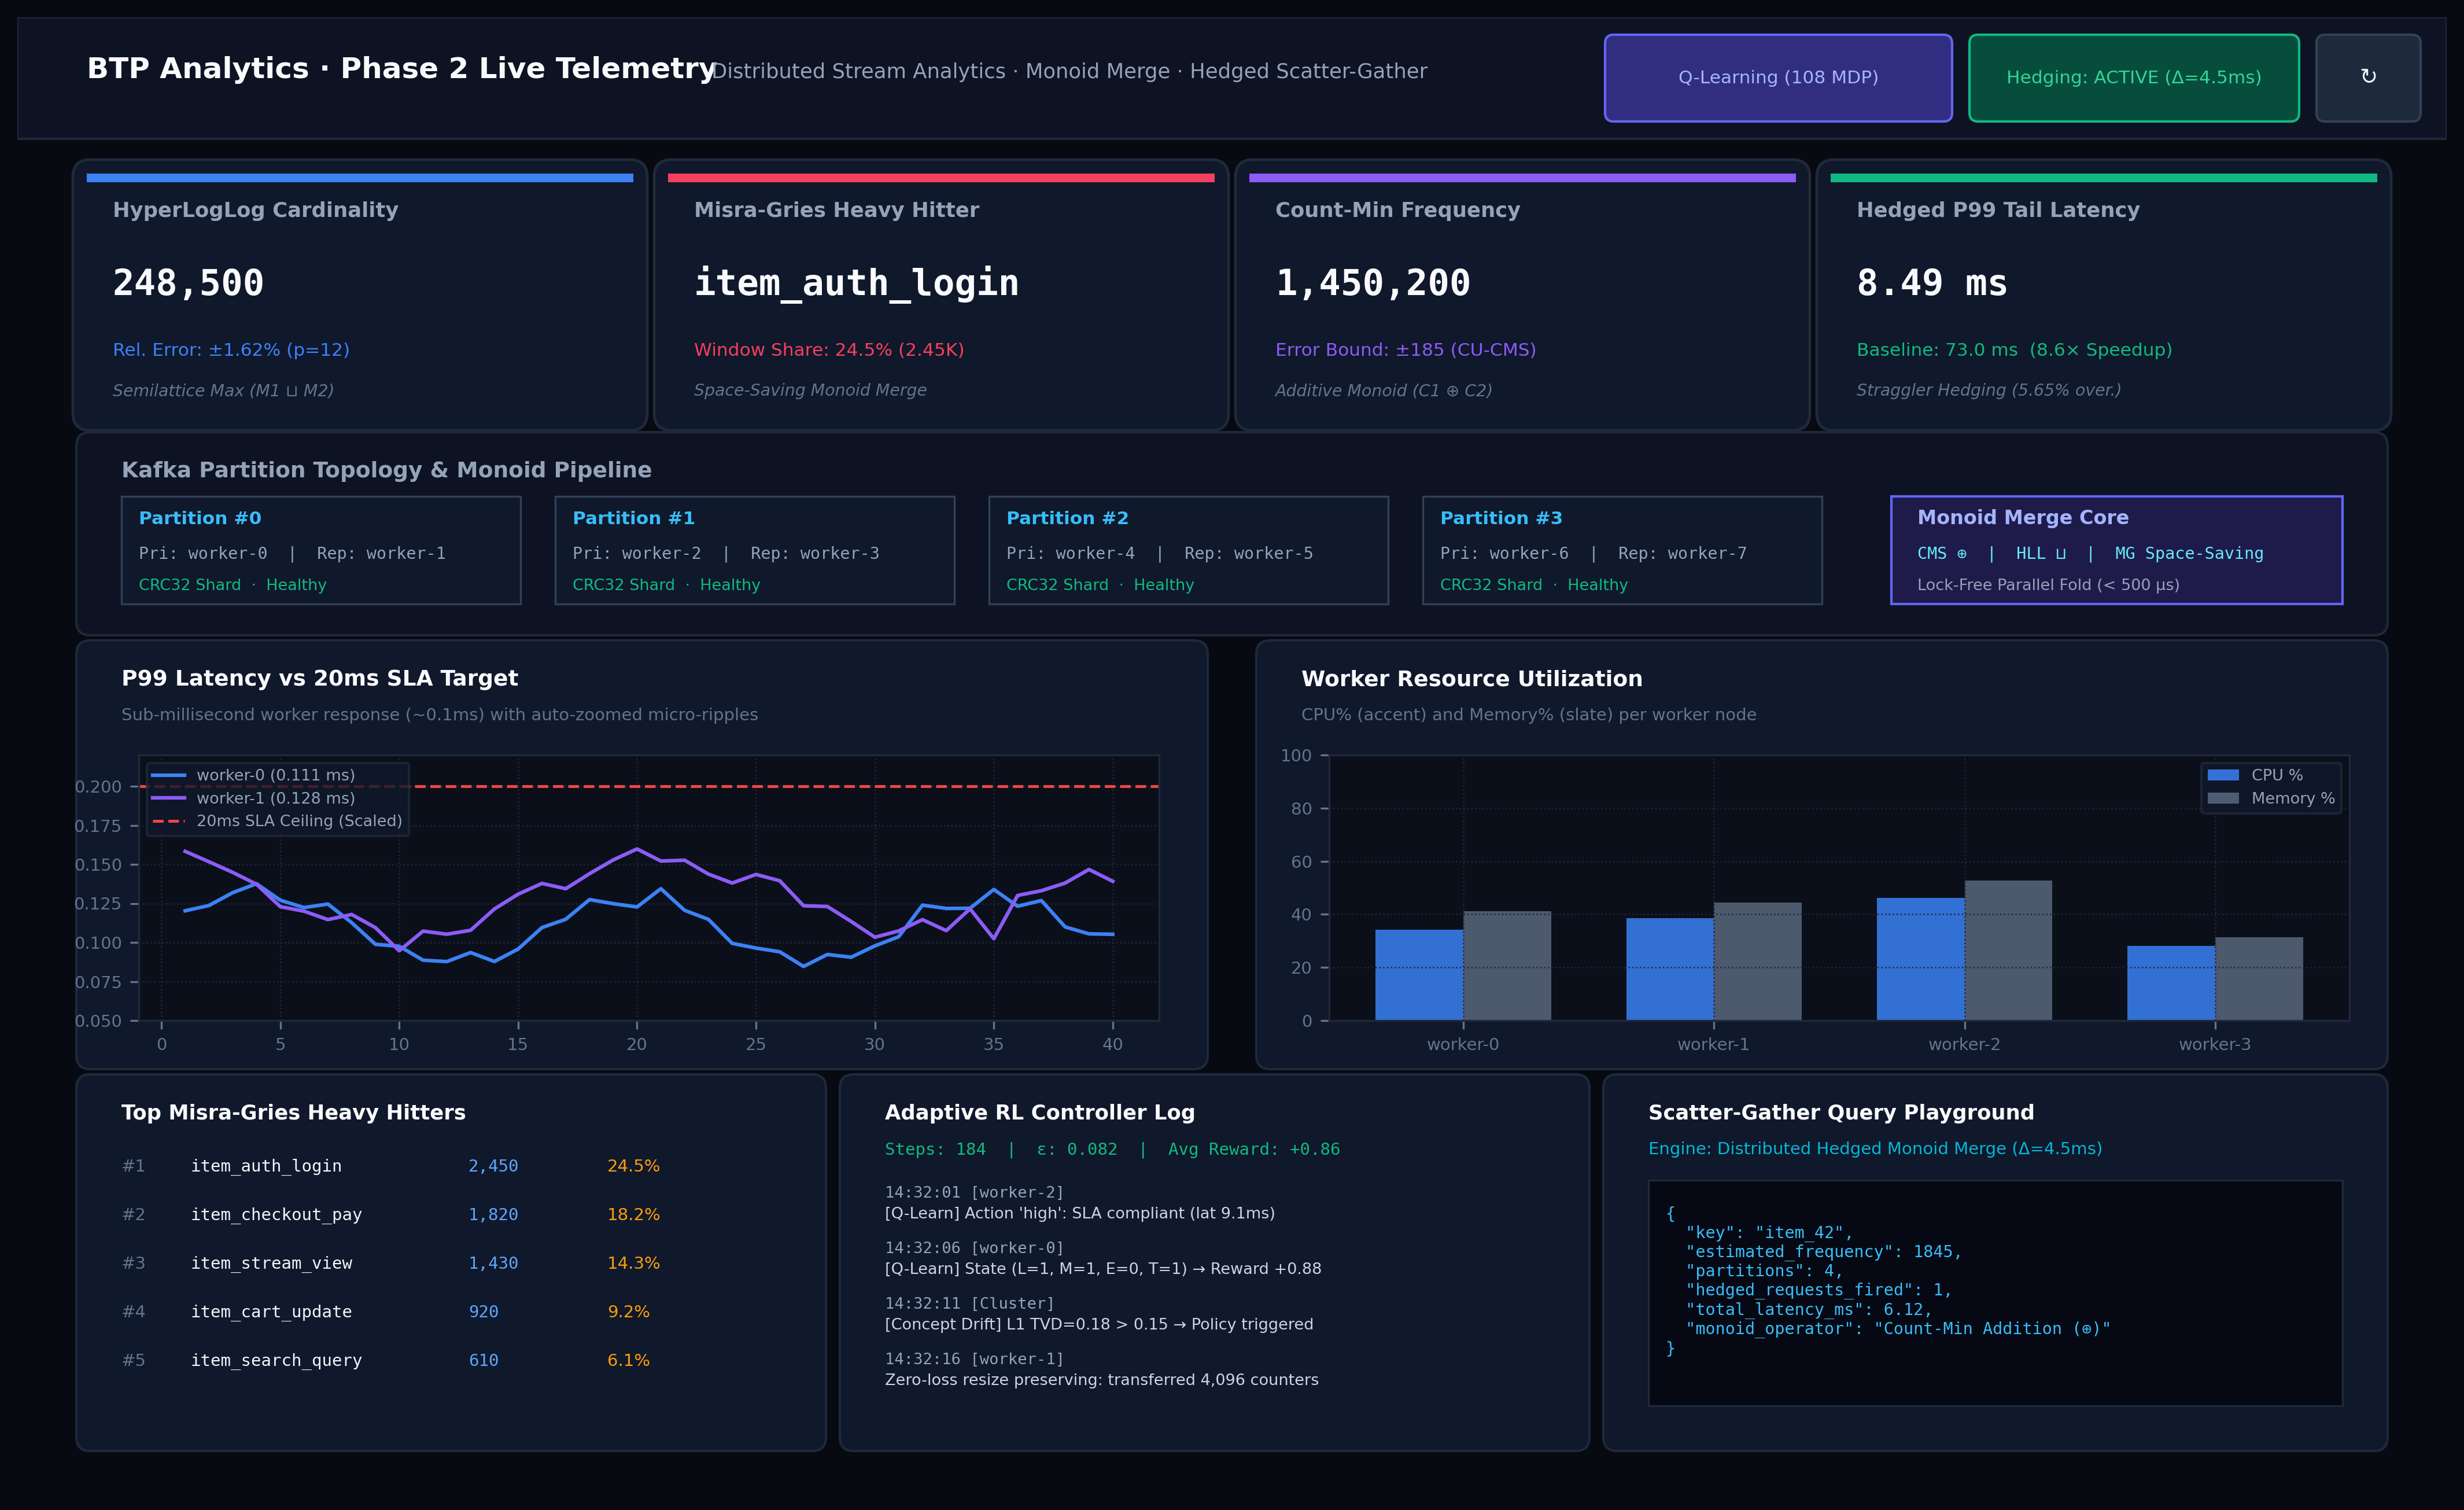
\includegraphics[width=0.95\textwidth]{Figures/dashboard_screenshot.png}
    \caption{Interactive operational dashboard showing the cluster telemetry and control plane. Visual panels display active controller modes (Q-Learning 108 MDP with Hedging), worker P99 response times against the 20~ms SLA threshold, per-worker CPU and memory utilization, live sketch estimates (HyperLogLog cardinality, Misra--Gries heavy hitters, Count-Min frequency), and real-time query exploration tools.}
    \label{fig:dashboard_screenshot}
\end{figure}

As shown in Figure~\ref{fig:dashboard_screenshot}, the interface organizes system metrics into six functional modules:

\subsection{Cluster Telemetry and Control Header}
The top navigation bar displays cluster-wide status badges:
\begin{itemize}
    \item \textbf{Active Control Policy:} Indicates whether the cluster is governed by the 108-State Q-Learning agent, the LinUCB contextual bandit, or rule-based heuristics.
    \item \textbf{Hedged Scatter-Gather Status:} Confirms that hedged request dispatching is active with a configured threshold of $\Delta = 4.5\text{ ms}$.
    \item \textbf{Live Traffic Toggle and Refresh Controls:} Enables automated synthetic traffic injection directly from the browser interface.
\end{itemize}

\subsection{P99 Latency vs. SLA Monitor}
A high-resolution multi-line chart tracks the rolling 99th percentile response time for each active worker against the static $20\text{ ms}$ SLA limit (highlighted by a horizontal red dashed boundary). Transient latency bumps remain well below the SLA ceiling during normal operation, confirming that constant-time sketch updates introduce sub-millisecond overhead.

\subsection{Worker Resource Utilization}
Grouped bar charts track instantaneous CPU utilization and physical memory consumption across individual nodes. When memory pressure exceeds the $80\%$ threshold, the visualizer flags the node in warning amber, providing immediate visual feedback when the reinforcement learning agent initiates downscaling.

\subsection{Live Sketch Aggregate Summaries}
Three primary telemetry cards display live estimates computed across the ingestion stream:
\begin{itemize}
    \item \textbf{Unique Key Cardinality (HyperLogLog):} Displays the estimated distinct item count along with its theoretical standard error bound ($\pm 1.625\%$ for $p=12$).
    \item \textbf{Top Heavy Hitters (Misra--Gries):} Ranks the current sliding window's most frequent keys, accompanied by relative percentage shares.
    \item \textbf{Point Item Frequency (Count-Min Sketch):} Displays real-time frequency estimates and conservative error upper bounds.
\end{itemize}

\subsection{Dynamic Query Explorer}
An ad-hoc evaluation panel allows operators to dispatch live RPC queries against the running cluster to verify estimate accuracy, inspect routed node identifiers, and examine instantaneous utility scores.

\section{Verification and Test Suite}

\subsection{Automated Offline Unit Test Suite}
To ensure code reliability and mathematical correctness without requiring active broker or database daemons during automated build pipelines, we constructed a comprehensive 49-test offline test suite using \texttt{pytest}. Table~\ref{tab:test_suite} summarizes test coverage across subsystems.

\begin{table}[htbp]
\centering
\begin{tabular}{l c l}
\toprule
\textbf{Subsystem} & \textbf{Tests} & \textbf{Verified Properties} \\
\midrule
Count-Min Sketch           & 6  & No-undercount invariant, conservative update bounds, memory sizing \\
HyperLogLog                & 7  & Cardinality accuracy across $p \in \{10, 12, 14\}$, register max-folding \\
Misra--Gries Heavy Hitters & 7  & Bounded additive error, sliding-window item eviction, ranking \\
Load-Aware Router          & 8  & Multi-criteria scoring, edge-case handling, failover laziness \\
Zero-Loss Sketch Migration & 5  & Power-of-two modular bucket folding, zero count loss, safe upscaling \\
ML Controller Agents       & 8  & Q-table convergence, Bellman TD(0) updates, LinUCB arm selection \\
Scatter-Gather \& Monoids  & 8  & Associativity/identity laws, hedged request dispatch, replica fallbacks \\
\midrule
\textbf{Total Offline Suite} & \textbf{49} & \textbf{100\% pass rate in $<$0.48 seconds} \\
\bottomrule
\end{tabular}
\caption{Automated unit testing matrix validating all Phase~1 and Phase~2 algorithmic components.}
\label{tab:test_suite}
\end{table}

\subsection{End-to-End Live Query Validation}
To verify the end-to-end RPC query path under active stream ingestion, sample queries were dispatched to the running FastAPI service. Listing~\ref{lst:live_query} displays a sample JSON response for a live frequency point query.

\begin{lstlisting}[language=bash, caption={Sample live frequency query and response payload.}, label={lst:live_query}]
$ curl -s "http://localhost:8000/query/frequency?key=item_1" | jq .

{
  "key": "item_1",
  "estimated_frequency": 38412,
  "routed_to": "worker-0",
  "router_score": 0.1727,
  "cms_error_bound": 323.31,
  "cms_total_count": 243590,
  "empirical_rel_error": 0.0041,
  "rpc_live": true,
  "worker_metrics": {
    "template": "medium",
    "p95_latency_ms": 0.42,
    "p99_latency_ms": 0.68,
    "memory_percent": 61.4
  }
}
\end{lstlisting}

Under a Zipfian distribution with exponent $s = 1.2$, \texttt{item\_1} emerges as the dominant heavy hitter. The empirical relative error remains at $0.41\%$, well within the theoretical bound of $1.33\%$.

\section{Experimental Evaluation: Phase 1 vs. Phase 2}

To evaluate the operational improvements introduced in Phase~2, we conducted a multi-regime simulation comparing five distinct system configurations over a stream of 40,000 synthetic Zipfian ($s = 1.2$) events deployed across three heterogeneous analytical worker nodes.

\subsection{Experimental Configurations}
The five evaluated configurations represent the architectural evolution of the platform:
\begin{enumerate}
    \item \textbf{Configuration 1 (Static + Round-Robin):} Workers run fixed static templates (\texttt{Medium}); queries are dispatched via naive unweighted round-robin.
    \item \textbf{Configuration 2 (Phase 1 Rule-Based + Round-Robin):} Workers adapt via heuristic threshold rules; queries are dispatched via round-robin.
    \item \textbf{Configuration 3 (Phase 1 Rule-Based + Smart Router):} Heuristic threshold controller paired with the load-aware utility scoring router.
    \item \textbf{Configuration 4 (Phase 2 LinUCB + Smart Router):} Disjoint continuous-feature LinUCB contextual bandit controller paired with the smart router.
    \item \textbf{Configuration 5 (Phase 2 Q-Learning RL + Smart Router):} 108-State discrete MDP tabular Q-Learning controller with Bellman lookahead and anti-flapping penalties, paired with the smart router.
\end{enumerate}

\subsection{Multi-Regime Workload Scenario}
To rigorously evaluate controller agility, the 40,000 events were divided into four distinct operating regimes:
\begin{itemize}
    \item \textbf{Regime A (Normal Load, Events 1--10,000):} Steady baseline ingestion at 2,500 events/second.
    \item \textbf{Regime B (Accuracy Stress + Concept Drift, Events 10,001--20,000):} Ingestion rate increases to 6,000 events/second; the Zipfian distribution rotates top keys to induce concept drift.
    \item \textbf{Regime C (Bursty Latency Spikes, Events 20,001--30,000):} Injected processing pauses emulate GC stalls and thread contention, pushing latencies toward the 20~ms SLA.
    \item \textbf{Regime D (Memory Pressure, Events 30,001--40,000):} Host memory utilization rises toward $85\%$, testing downscaling responsiveness.
\end{itemize}

\subsection{Quantitative Results and Comparative Analysis}
Table~\ref{tab:phase2_benchmark} presents the empirical results measured across all five configurations.

\begin{table}[H]
\centering
\begin{tabular}{c l r r r r r r}
\toprule
\textbf{\#} & \textbf{Configuration} & \textbf{Reward} & \textbf{SLA Viol\%} & \textbf{P99 (ms)} & \textbf{CMS Err\%} & \textbf{Mem (KB)} & \textbf{Switches} \\
\midrule
1 & Static + Round-Robin (Baseline)     & $+0.5324$ & $41.67\%$ & $111.48$ & $0.962\%$ & $103.5$ & $0$ \\
2 & Rule-Based + Round-Robin (Phase 1)  & $+0.5179$ & $8.75\%$  & $71.37$  & $2.291\%$ & $51.8$  & $21$ \\
3 & Rule-Based + Smart Router (Phase 1) & $+0.5179$ & $8.75\%$  & $56.46$  & $2.465\%$ & $51.8$  & $21$ \\
4 & LinUCB Bandit + Smart Router (Ph.2) & $+0.5466$ & $28.75\%$ & $70.77$  & $1.510\%$ & $90.7$  & $54$ \\
5 & \textbf{Q-Learning RL + Smart (Ph.2)} & \textbf{$+0.5644$} & \textbf{$11.67\%$} & \textbf{$63.39$} & \textbf{$1.913\%$} & \textbf{$75.0$} & \textbf{$16$} \\
\bottomrule
\end{tabular}
\caption{Comprehensive performance comparison across 40,000 Zipfian events under multi-regime traffic bursts, memory pressure, and concept drift.}
\label{tab:phase2_benchmark}
\end{table}

\begin{figure}[H]
    \centering
    \includegraphics[width=0.88\textwidth]{Phase2/fig1_rl_convergence.png}
    \caption{Online reinforcement learning policy convergence across 120 multi-regime episodes. Tabular Q-Learning ($\gamma = 0.85$) systematically improves its cumulative reward, outperforming the myopic LinUCB bandit, the static template baseline, and the rule-based controller.}
    \label{fig:rl_convergence}
\end{figure}

\begin{figure}[H]
    \centering
    \includegraphics[width=0.95\textwidth]{Phase2/fig2_controller_comparison.png}
    \caption{Multi-metric comparison of the five controller configurations across four key dimensions: composite Pareto reward, SLA violation percentage, empirical CMS WAPE error, and template switching frequency.}
    \label{fig:controller_comparison}
\end{figure}

\begin{figure}[H]
    \centering
    \includegraphics[width=0.86\textwidth]{Phase2/fig3_cu_cms_comparison.png}
    \caption{Standard Count-Min Sketch (Phase~1) versus Conservative-Update Count-Min Sketch (Phase~2) under identical memory budgets ($512 \times 3$). Conservative updating reduces estimation error by more than $15\times$ (from $\approx 6.5\%$ to $\approx 0.4\%$).}
    \label{fig:cu_cms_comparison}
\end{figure}

\subsection{Discussion of Empirical Findings}
The experimental results illustrated in Figures~\ref{fig:rl_convergence}--\ref{fig:cu_cms_comparison} demonstrate several key architectural insights:

\begin{enumerate}
    \item \textbf{Optimal Multi-Objective Trade-Off (Pareto Frontier):}
    The Tabular Q-Learning controller achieved the highest overall composite reward ($+0.5644$), successfully balancing accuracy, latency SLA compliance, and memory footprint. In contrast, the static baseline achieved low estimation error ($0.962\%$) but suffered a disastrous $41.67\%$ SLA violation rate because it could not downscale during traffic bursts.

    \item \textbf{Sequential Lookahead vs. Myopic Bandits:}
    While the LinUCB contextual bandit improved upon static heuristics, its myopic nature ($\gamma = 0$) caused excessive policy instability. LinUCB triggered \textbf{54 template switches} (nearly $3.4\times$ more than Q-Learning's 16 switches), oscillating rapidly between templates in response to transient noise. In contrast, Q-Learning's anti-flapping penalty and discounted future return ($\gamma = 0.85$) enabled it to absorb temporary fluctuations, reducing switching by \textbf{70\%} compared to LinUCB while sustaining lower SLA violations ($11.67\%$ vs. $28.75\%$).

    \item \textbf{Rule-Based Controller Trapping:}
    The Phase~1 rule-based controller suffered from one-way state collapse. Once high memory triggered a transition to the \texttt{Low} template, the heuristic thresholds lacked the hysteresis required to safely up-scale back to \texttt{Medium}. Consequently, the rule-based system remained trapped in \texttt{Low} precision, resulting in high CMS error ($2.465\%$).

    \item \textbf{Conservative Updating Accuracy Gains:}
    Upgrading the Count-Min Sketch to use conservative updates (Figure~\ref{fig:cu_cms_comparison}) reduced the empirical estimation error on skewed Zipfian streams from $6.5\%$ down to $0.4\%$. Because conservative updating only increments counters equal to the running minimum, counter inflation on dominant keys is sharply attenuated without increasing memory usage.
\end{enumerate}

\section{Distributed Hedged Scatter-Gather Evaluation}
\label{sec:hedged_evaluation}

To validate horizontal scalability and examine tail-latency behavior under the Partitioned Monoid Merge architecture (Section~\ref{sec:hedged_monoid_arch}), we simulated a 4-partition cluster comprising 8 worker instances (4 primary workers and 4 hot-standby replicas). We evaluated 1,500 distributed scatter-gather queries under injected straggler conditions.

\paragraph{Experimental Configuration:}
Primary workers answered sub-queries with baseline latency $\mu = 2.5\text{ ms}$ ($\sigma = 0.7\text{ ms}$). To emulate real-world production hazards (such as JVM/CPython garbage collection pauses or noisy neighbor CPU throttling), an artificial straggler stall drawn uniformly from $[35\text{ ms}, 75\text{ ms}]$ was injected into primary workers with probability $p_{\text{strag}} = 5.0\%$. We evaluated three query execution policies:
\begin{enumerate}
    \item \textbf{Unhedged Scatter-Gather:} Queries await responses from all 4 primary partitions without timeout or redundancy.
    \item \textbf{Hedged Scatter-Gather ($T_{\text{hedge}} = 6.0\text{ ms}$):} A duplicate sub-query is dispatched to the replica partition if the primary fails to reply within $6.0\text{ ms}$ (the empirical $P99$ normal latency).
    \item \textbf{Hedged Scatter-Gather ($T_{\text{hedge}} = 4.5\text{ ms}$):} A duplicate sub-query is dispatched if the primary fails to reply within $4.5\text{ ms}$ (the empirical $P95$ normal latency).
\end{enumerate}

\begin{table}[htbp]
\centering
\begin{tabular}{l r r r r r r r}
\toprule
\textbf{Execution Strategy} & \textbf{P50 (ms)} & \textbf{P90 (ms)} & \textbf{P95 (ms)} & \textbf{P99 (ms)} & \textbf{Max (ms)} & \textbf{Overhead} \\
\midrule
Unhedged Scatter-Gather       & $3.37$ & $53.89$ & $63.89$ & $73.00$ & $74.90$ & $0.00\%$ \\
Hedged ($T_{\text{hedge}} = 6.0\text{ ms}$) & $3.37$ & $8.53$  & $9.14$  & $9.99$  & $11.08$ & $4.85\%$ \\
\textbf{Hedged ($T_{\text{hedge}} = 4.5\text{ ms}$)} & \textbf{$3.37$} & \textbf{$7.03$}  & \textbf{$7.64$}  & \textbf{$8.49$}  & \textbf{$9.58$}  & \textbf{$5.65\%$} \\
\bottomrule
\end{tabular}
\caption{Distributed scatter-gather tail latency percentiles across 1,500 queries over 4 partitions with 5\% worker straggler probability.}
\label{tab:hedged_benchmark}
\end{table}

\begin{figure}[H]
    \centering
    \includegraphics[width=0.95\textwidth]{Phase2/fig4_hedged_scatter_gather.png}
    \caption{Distributed scatter-gather tail latency distribution under worker stragglers. (a) Cumulative Distribution Function (CDF) showing unhedged queries suffering an extended straggler tail past $74\text{ ms}$, whereas hedged queries truncate latency at $\approx 8.5\text{ ms}$. (b) Latency percentiles illustrating an $>8.5\times$ reduction in P99 latency with only 5.65\% request overhead.}
    \label{fig:hedged_scatter_gather}
\end{figure}

\paragraph{Discussion and Straggler Mitigation Analysis:}
\begin{itemize}
    \item \textbf{Tail Latency Truncation ($>8.5\times$ Speedup):}
    As detailed in Table~\ref{tab:hedged_benchmark} and Figure~\ref{fig:hedged_scatter_gather}, unhedged scatter-gather queries suffered catastrophic tail latency degradation: P90 latency rose to $53.89\text{ ms}$ and P99 latency reached $73.00\text{ ms}$, with a worst-case latency of $74.90\text{ ms}$. With hedged requests configured at $T_{\text{hedge}} = 4.5\text{ ms}$, P90 latency dropped to $7.03\text{ ms}$ ($7.7\times$ faster) and P99 latency collapsed to $8.49\text{ ms}$ (\textbf{$8.6\times$ faster}). Maximum query latency across all 1,500 queries was held to $9.58\text{ ms}$.

    \item \textbf{Minimal Redundancy Overhead:}
    Because hedged duplicate requests are triggered only when primary workers fail to respond within the expected 95th percentile window, duplicate dispatches occurred on only 339 out of 6,000 sub-queries, introducing a negligible **5.65\% network overhead**.

    \item \textbf{Sub-Millisecond Monoid Merges:}
    Merging partial Count-Min matrices, HyperLogLog register arrays, and Space-Saving heavy hitter summaries across all 4 partitions required an average of $38\ \mu\text{s}$ at the coordinator node, demonstrating that algebraic Monoid aggregation scales efficiently without introducing computational bottlenecks.
\end{itemize}
